\lab{Algorithms}{Matrix Operations and Algorithmic Complexity}{Matrices and Complexity}

\objective{This section explains how to create specific types of large matrices. It also introduces the concept of temporal complexity. Finally, it explores SciPy's special methods for working with sparse matrices.}

\section*{Temporal Complexity}

%{\bf The next two paragraphs are an alternate description of Big O, designed as a more intuitive approach, to help with Vol I (a more technical explanation would be in Vol II). Let me know what you think...}

%I am not sure that this is clear or precise enough.  I think that the previously written stuff with some easier problems may be better...

One of the most important questions in scientific computing is: How long will this operation take?  The concept of temporal complexity attempts to answer this question by determining how much time a function needs to operate on a given size of input.  For example suppose calculating the inverse of a matrix of size $n$ requires the following number of calculations.
%For this reason we often discuss algorithms in terms of their temporal complexity, which describes how long an operation takes in terms of the size of the input. For example, suppose calculating the inverse of a matrix of size $n$ requires the following number of calculations:
\[
f(n) = \frac{3n^3}{2} + 75n^2 + 250n + 30
\]
What is the most important part of this expression? When our input gets very large the only relevant term in this equation is $n^3$. For this reason we say that $f(n) \in O(n^3)$, or more commonly that $f(n)$ is $O(n^3)$ (spoken ``Big O of n cubed'' or ``Order of n cubed"). This notation is borrowed from analysis. This notation captures the salient behavior of our temporal complexity, or more precisely the growth rate we can expect of the execution time of our algorithm. We will discuss this concept later, but this is a simple introduction to the notion of complexity and Big O. Spatial complexity is the amount of memory an algorithm uses, and is defined similarly. 

\begin{comment}

Now that we have begun to study some more complex MATLAB expressions, it is prudent to have a basic notion of the complexity of the operations we are interested in executing.  Complexity theory is the study of the difficulty of computational problems.  What makes computing the sum of two integers easy, and what makes computing the inverse of a large matrix so difficult?  There is an entire field dedicated to answering such questions; in this work we only do a cursory examination to communicate the basic ideas and vocabulary.
	
	To begin, we use an example to illustrate what we are trying to accomplish.  There are occasions when one is willing to sacrifice precision in order to focus on more important features of the object of study.  For example, $f(x) = x^3 + \frac{sin(20x)}{10}$ produces a cubic function with a slight wobble.  In some applications that wobble may be a crucial detail, but in many cases the wobble will be irrelevant and only serves to distract from the salient features of the function.  We extend this example to algorithms.

	An algorithm is an ordered set of instructions.  Something simple like a recipe to bake a cake is an algorithm, but the only algorithms you will be dealing with here are MATLAB operations and programs.  To describe the complexity of an algorithm we use asymptotic notation called ``Big O.''  Big O makes us focus on salient features of the complexity of an algorithm while at the same time suppressing unnecessary details, much like we ignored the sine wobble in the previous example.  It has been said that using Big O is ``the art of knowing where to be sloppy and where to be precise.''
	
	With that introduction, we define Big O:
	
\begin{theorem}
	$f(x) = O(g(x))$ if and only if $\exists$ M $\in \mathbb{N}, x_0 \in dom(f)$ such that $|f(x)| \le M|g(x)|$ $\forall x > x_0$
 \end{theorem}
 
 This is an abuse of notation, we really should be saying that $f(x) \in O(g(x))$ since $O(g(x))$ is not a function but an equivalence class of functions.  Lamentably, using $=$ has become embedded into the culture, so there is not much to be done except make a note of the correct notation and move along.
 
 \begin{example}
 $x^2 = O(x^3)$ since $x^2 < x^3$ when $x > 1$
 \end{example}
 
 \begin{example}
 $x^3 + 3x^2 + x + 4 = O(x^3)$ since $x^3 + 3x^2 + x + 4 < 10x^3$ when $x > 1$
 \end{example}
 
  \begin{example}
 $x^2 + 10000x = O(x^2)$ since $x^2 + 10000x < 100000x^2$ for all x.
 \end{example}
 
You can see that when we talk about Big O of polynomials, we are simply dropping off lower order terms and ignoring coefficients.
% 
% (These problems may be too challenging)
% \begin{problem}
% Show that $O(\log{x}) \subset O(x) \subset O(x\log{x})$
% \end{problem}
% 
% \begin{problem}
% Show that $O(x^k) \subset O(x^{k+1})$
% \end{problem}
% 
% \begin{problem}
% Show that $O(x^p) \subset O(2^x)$ for all $p \in \mathbb{N}$
% \end{problem}
% 
	What does this have to do with computer programs?  Every algorithm executed on a computer corresponds to a function that returns the number of steps taken (and therefore the time) given an input of size n.  Certain problems can be solved with fewer steps, whilst others require many more.  For example, given two matrices of size n, it only takes about n steps to add the entries together and thus matrix addition is $O(n)$.  On the other hand, given a matrix of size $n$, it takes about $n^3$ steps to calculate its inverse, and thus inverting a matrix is $O(n^3)$.  There is something inherently more difficult about inverting a matrix; there is complexity that simply isn't there with the straightforward operation of addition.
%	
%	We will return to complexity analysis after we know a little bit more about writing our own scripts and functions.
\end{comment}	
	
\section*{Advanced Matrix Tools}

We now introduce a few different ways to build matrices. Two important methods available for building matrices are \li{zeros()} and \li{ones()}. These commands allow us to build matrices populated entirely with zeros or ones, respectively. For example, to build a 3-vector filled with zeros we enter the following command:

\begin{lstlisting}
: import scipy as sp
: sp.zeros((3,1))
array([[ 0.],
       [ 0.],
       [ 0.]])
\end{lstlisting}

To find additional options for these methods, you can use the help system.

%Better explanation and an example or two should go here.

One important use of the \li{zeros()} method is to allow us to pre-allocate memory. Pre-allocation is simply the practice of reserving a chunk of memory for later use. We can always add more space to a matrix using the methods we learned in lab 1, but this requires many extra internal operations because of way arrays are stored in memory. Thus, it is generally faster to allocate a matrix with its final size and modify its values rather than building an array as you go.

%Problem here comparing pre-allocation vs. no pre-allocation.  There should be several orders of magnitude difference.

% Perhaps more of a segue here?

Table 1.3 gives a few commands that allow us to build types of useful matrices.

\begin{table}[h!]

\begin{center}

    \begin{tabular}{|l|p{4cm}|l|}

    \hline

    Function & Description & Usage \\

    \hline

    \li{eye()} & Identity matrix & sp.eye(m, n)\\

    \li{zeros()} & Zero matrix & sp.zeros((m, n))\\

    \li{ones()} & One matrix & sp.ones((m, n))\\

    \li{diag()} & Building (or retrieving) along a diagonal&\\

    \li{linalg.toeplitz()} & Matrix with constant diagonals & la.toeplitz()\\

    \li{linalg.triu()} & Upper triangular&\\
    
    \li{linalg.tril()} & Lower triangular&\\
    
    \li{rand} & Psuedo-random matrix, uniformly distributed&\\

   \li{randn} & Psuedo-random matrix, normally distributed&\\

   \li{random.randint()} & Psuedo-random matrix, uniformly distributed integers & sp.random.randint()\\
    
    \li{tile()} & Copy across a given dimension & sp.tile(A, reps)\\

    \hline

    \end{tabular}
	\caption{Special matrix creation commands}

\end{center}
\end{table}

For example, suppose that we want to create a matrix with $-2$ on the diagonal, and ones on the super and sub diagonal. We can do this by using the following command:

\begin{lstlisting}
: from scipy import linalg as la
: la.toeplitz([-2,1,0])
array([[-2,  1,  0],
       [ 1, -2,  1],
       [ 0,  1, -2]])
\end{lstlisting}

This matrix is useful because it numerically approximates the second derivative of a function. We investigate some properties of this matrix in Problem 6 of this lab, and explain more about this matrix later.

\begin{problem}
Use the \li{diagflat()} method to create the following matrices. All of these matrices should be easily scalable (i.e., only minor modification would be required to change the size).
\[
\begin{pmatrix}
1&2&3&4&5\\
0&1&2&3&4\\
0&0&1&2&3 \\
0&0&0&1&2 \\
0&0&0&0&1 \\
\end{pmatrix}
\hspace{8mm}
\begin{pmatrix}
1&1/2&1/3 & 1/4 &1/5\\
1/2&1&1/2&1/3&1/4\\
1/3&1/2&1&1/2&1/3 \\
1/4&1/3&1/2&1&1/2 \\
1/5&1/4&1/3&1/2&1 \\
\end{pmatrix}
\]
\end{problem}

\begin{problem}
Create the matrices from Problem 1 using the methods \li{linalg.toeplitz()} or \li{linalg.triu()}. Which method is easier? Now use whichever command is easiest to create the matrix:
\[
\begin{pmatrix}
1&0&0&0&0\\
0&2&0&0&0\\
0&0&3&0&0 \\
0&0&0&4&0 \\
0&0&0&0&5 \\
\end{pmatrix}
\]
\end{problem}
 
\begin{comment}
\begin{problem}
Write a function that will create a matrix of size $n$ that has ones on the diagonal and has normally-distributed random entries in the last two columns and the last two rows.
%Do this in one line using the commands from this section and matrix building techniques from Lab 1.1.
\end{problem}
\end{comment}

\section*{Sparse Matrices}
In this section we discuss how sparse matrices are used and constructed. A sparse matrix is a matrix that has few non-zero entries (where few is generally relative to the number of entries in the matrix).  SciPy has several different ways of storing sparse matrices.  Each way has it pros and cons (the reader is encouraged to read the help for way).

\begin{table}[h!]

\begin{center}

    \begin{tabular}{|c|c|}

    \hline

    Function & Description \\

    \hline

    \li{sparse.bsr()} & Compressed Block Sparse Row\\
    
    \li{sparse.coo()} & Coordinate\\
    
    \li{sparse.csc()} & Compressed Sparse Column\\
    
    \li{sparse.csr()} & Compress Sparse Row\\
    
    \li{sparse.dia()} & Sparse Diagonal\\
    
    \li{sparse.dok()} & Dictionary of Keys\\
    
    \li{sparse.lil()} & Linked List\\

    
    \hline

    \end{tabular}
        \caption{Sparse matrix representations in SciPy}
\end{center}
\end{table}

Type the following into IPython.
\begin{lstlisting}
: from scipy import sparse as spar
: A = sp.diagflat([2,3,4])
: B = spar.csc_matrix(A)
: C = B.todense()
\end{lstlisting}

Notice that the matrix $A$ has only three non-zero entries, and so we can consider it sparse. In memory, an array stores a bit of data (be it an integer, float, or complex number) each entry, meaning that a $3 \times 3$ matrix requires a total 9 blocks of memory. However, if we leverage the sparsity of $A$ we realize that we only need to store 3 numbers. The \li{sparse} methods do exactly this: they store only the non-zero entries and their locations in the matrix. No longer are we working with array.  SciPy has many methods for performing operations on sparse arrays.  To convert back to a dense matrix, we use the \li{.todense()} property of the sparse matrix.  We can also convert between the different types sparse arrays.

We remark that if you want to make a sparse diagonal matrix, the
best way to do it isn't to use \li{diagflat()} followed by \li{sparse},
it's actually better to use the \li{sparse.spdiags()} method:
\begin{lstlisting}
: spar.spdiags([2,3,4],0,3,3)
\end{lstlisting}

This is because oftentimes when we are using sparse matrices we are dealing with matrices that are too large to be handled efficiently by python when represented in full form.

\section*{Banded Matrices}
A banded matrix is one whose only non-zero entries are diagonal
strips.  For example, the matrix
\[
A = \begin{pmatrix} 1&2&0&0\\3&4&5&0\\0&6&7&8\\0&0&9&10
\end{pmatrix}
\]
is banded because there are three nonzero diagonals.  This
particular type of banded matrix is called a tri-diagonal matrix.

You can easily create banded matrices using the \li{diagflat()} method.  For example, the matrix $A$ above can be created by
entering
\begin{lstlisting}
: sp.diagflat([3,6,9],-1) + sp.diagflat([1,4,7,10],0) + sp.diagflat([2,5,8],1)
\end{lstlisting}

Often a better way to create a tri-diagonal is it use the \li{spar.spdiags()} method. This is because many diagonal matrices are sparse. For example, we create the same matrix in Python (while designating that it is sparse) using the command:
\begin{lstlisting}
: Z = sp.array([[3, 1, 0],[6, 4, 2],[9, 7, 5],[0,10,8]]).T
: spar.spdiags(Z,[-1,0,1],4,4)
\end{lstlisting}

For more information, check the documentation by typing \li{spar.spdiags?}. For example we create a tri-diagonal array with uniformly distributed random entries.  This example also demonstrates the efficiency of using sparse arrays.
\begin{lstlisting}
: B = sp.rand(3,10000)
: A = spar.spdiags(B,range(-1,2),10000,10000)
: denseA = A.todense()  #only do this step if you have _lots_ of memory!
: A.data.nbytes
240000          #about 0.24MB of memory
: denseA.nbytes
800000000       #about 762.9MB of memory!
\end{lstlisting}


We can't use the \li{full} command in this case because the computer will almost certainly run out of memory (the matrix is $10,\!000 \times 10,\!000$). However, we can still visualize this matrix using the \li{plt.spy()} command from matplotlib, which essentially shows the location of non-zero entries in a matrix. The output of \li{plt.spy(A)} in this case is shown in Figure 1.2:

%change to plt figure
\begin{figure}[h!]
\begin{center}
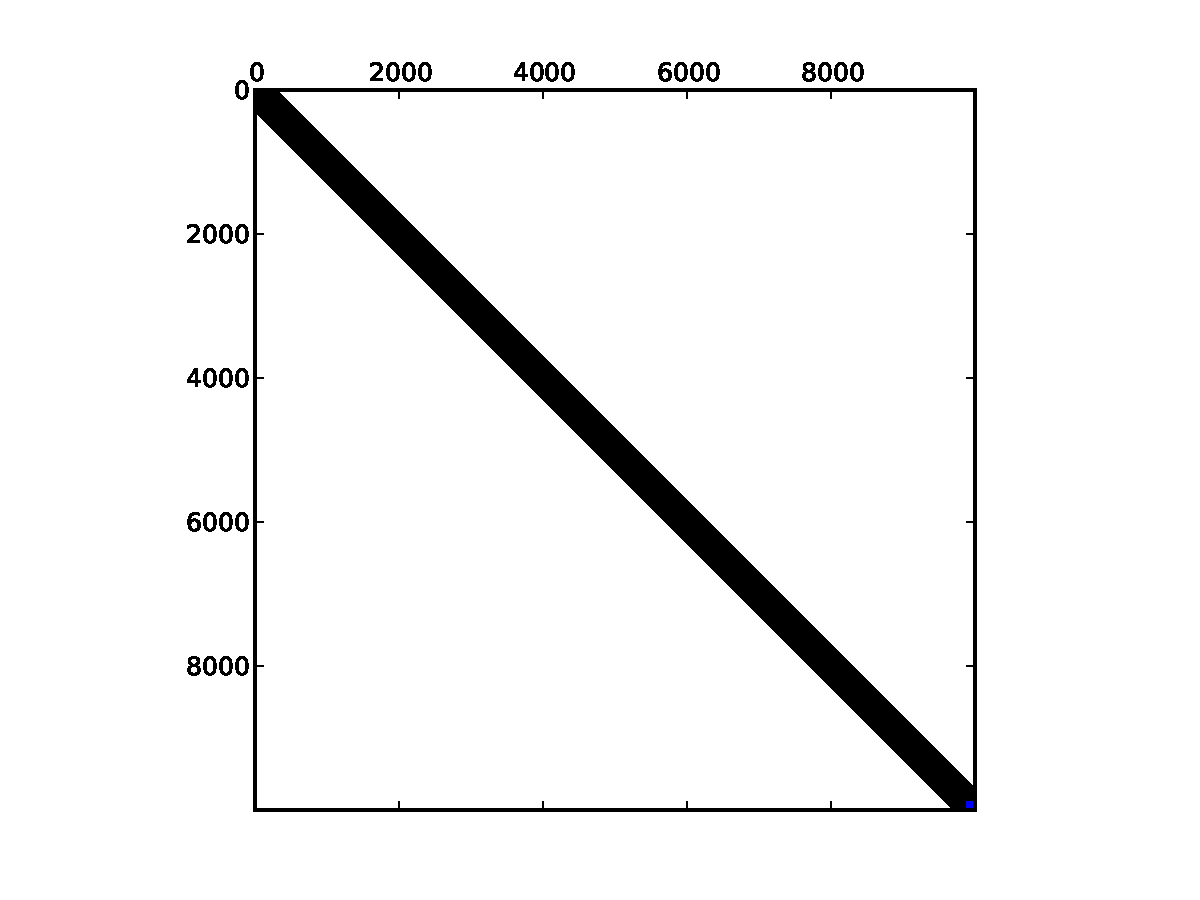
\includegraphics[scale = .5]{./Figures/spy}
\end{center}
\caption{The output of the \li{spy} command.}
\end{figure}

\section*{Using Sparse Matrices}

Consider the linear system $A x = b$, where $A$ is a
 $100,\!000\times 100,\!000$ tri-diagonal matrix.  To store a full
matrix of that size in your computer, it would normally require 10
billion double-precision floating-point numbers.  Since it takes 8
bytes to store a double, it would take roughly 80GB to store the
full matrix.  For most desktop computers, that fact alone makes the
system numerically prohibitive to solve. The temporal complexity of the problem is even more problematic. Methods for directly solving an arbitrary linear system are usually $O(n^3)$.  As
a result, even if the computer could store an 80GB matrix in RAM, it
would still take several weeks to solve the system.  However, since
we don't have computers with that much available RAM, most of the
matrix would have to be stored on the hard drive, so the computation
would probably take between $6$ months to a year.

The point is that even the next generation of computers will
struggle with solving arbitrary linear systems of this size in a
reasonable period of time.  However, if we take advantage of the
sparse structure of the tri-diagonal matrix, we can solve the linear
system, even with a modest modern computer.  This is because all of
those zeros don't need to be stored and we don't need to do as many
operations to row reduce the tri-diagonal system.

Let's first compute the spatial complexity of the above system when
considered as a sparse matrix.  There are three diagonals that have
roughly $100,\!000$ non-zero entries.  That's $300,\!000$
double-precision floating point numbers, which is about 2.4 MB (Less
storage than your favorite song).  As a result, it will easily
fit into the computer's RAM.  Furthermore, the temporal complexity for solving
a tri-diagonal matrix is $O(n)$. Let's see how long it takes to
solve the system for random data:

\begin{lstlisting}
: from scipy.sparse import linalg as sparla
: from timer import timer
: D = sp.rand(3, 100000)
: b = sp.rand(1, 100000)
: A = spar.spdiags(D,[-1,0,1],100000,100000)
: def solSys():
....: return sparla.spsolve(A,b)
: with timer() as t:
....: t.time(solSys)
....: t.printTimes()
\end{lstlisting}

\begin{problem}
Write a function that returns a full $n\times n$
tri-diagonal array with $2$'s along the diagonal and $-1$'s along
the two sub-diagonals above and below the diagonal. Hint: Use the \li{la.toeplitz()} method. Note that this is the second derivative matrix that we discussed at the beginning of this lab.
\end{problem}

\begin{problem}
Write another function that builds the same array as above, but as a sparse array. You must build this as a sparse matrix from the beginning. Hint: Use the \li{spar.spdiags()} method.
\end{problem}

\begin{problem}
Solve the linear system $Ax = b$ where $A$ is the $n\times n$
tri-diagonal array from the above two problems and $b$ is randomly
generated.  How high can you go for each method?  Make a table for
several different values of $n$ and the time it took to solve for
each run.  What conclusions can you draw?
\end{problem}

\begin{problem}
Using the sparse array above and the method \li{la.eigs()}, calculate the smallest eigenvalue $\lambda$ of the array as the array's size goes to infinity. What value does $\lambda n^2$ approach?  Hint: It's the square of an important number. This is related to operator theory: the second derivative operator has this eigenvalue in certain cases.
\end{problem}

\section*{Other Sparse Commands}

One important method of sparse array objects is the \li{nonzero()} method, which is related to the number of nonzero entries in an array.  This number is important because it is an indicator of the amount of time and space that is required to operate on the sparse array. You should be aware that there is some overhead to using and storing the sparse array data structure. Sparsely represented arrays are very beneficial when the number of nonzero entries is relatively small compared to the total number of entries. When the array has many nonzero entries, a sparse representation becomes disadvantageous. To see this, create and execute a script with the following code:
\begin{lstlisting}
: A = sp.rand(600,600); B = spar.csc_matrix(A)
: def square(A): return sp.power(A, 2)
: with timer() as t:
....: t.time(square, A)
....: t.time(square, B)
\end{lstlisting}

Run the script and note the two different runtimes. Notice that it takes much longer to square the sparse array. This is because the sparse array data structure is optimized for arrays that are actually sparse. The array $A$ is entirely nonzero. Thus, you incur the overhead of the sparse array representation without any benefits since there are no entries you are not required to store or compute. To summarize, only use a sparse array when your array is in fact sparse. Using sparse arrays for mostly nonzero arrays will negatively impact performance and memory requirements.


Just as with dense arrays, we can pre-allocate sparse arrays. Sometimes it is necessary to create sparse matrices that do not have a nice banded pattern.  We initialize a sparse array just like any other array.  The most efficient sparse array for pre-allocation is LIL.  Once you are done constructing you sparse array and wish to perform calculations, you should convert to a more efficient sparse array (CSR or CSC).
\begin{lstlisting}
: Z = spar.lil_matrix((400,300))
<400x300 sparse matrix of type '<type 'numpy.float64'>'
        with 0 stored elements in LInked List format>
: Z[1,34] = 23
: Z[23,32] = 56
: Z[2,:] = 13.2
\end{lstlisting}

This code snippet creates a $400 \times 300$ LIL sparse array.  We can then work with the sparse array as though it were a dense array.  When the array is initialized all of the entries
are assumed to be zero.